\documentclass[11pt,a4paper]{article}
\usepackage[left=24mm,top=4.0cm,right=24mm,bottom=4.0cm]{geometry}
\usepackage[utf8]{inputenc}
\usepackage{graphicx}
\usepackage{caption}

\newtheorem{1}{Definição}
\newtheorem{2}{Análise}
\newtheorem{3}{Observação}

\title {Projeto Álgebra Linear \\[1ex] \large Análise dos Componentes Principais em um Conjunto de Dados}

\author{Gabriel Luiz dos Santos Silva\\
João Pedro Borges Baeta
}

\date{06 dezembro 2022}

\begin{document}

\maketitle


%%%%%%%%%%%%%%%%%%%%%%%%%%%%%%%%%%%%%%%%%
% Introdução, Extração e Itens
%%%%%%%%%%%%%%%%%%%%%%%%%%%%%%%%%%%%%%%%%

\section{Introdução} \hspace{0.6cm}
Este trabalho contém a análise de informações correspondente ao custo de vida em quase 5000 cidades espalhadas pelo mundo. Toda a análise pode ser vista no JupyterNotebok chamado "principal-book-analysis.ipynb" no Github.

\begin{description}
\item[Github:] https://github.com/gabrielluizone/Principal-Component-Analysis
\end{description}

Os dados foram extraídos da base de dados do site Numbeo (https://numbeo.com), onde se disponibiliza, por meio da contribuição dos mais de 700 mil contribuidores, o custo de vida de mais de 10 mil cidades espalhadas pelo planeta.  Os dados estão disponível para download no Kaggle pelo usuário mvieira101, chamado "global-cost-of-living".

\begin{3} \normalfont
Ao todo, foram 54 itens utilizados para o cálculo em dólar do custo de vida nas cidades espalhadas pelo mundo. Para não haver a poluição da página, os itens podem ser visto na pasta "data" contendo o dicionário das colunas no Github.
\end{3}

%%%%%%%%%%%%%%%%%%%%%%%%%%%%%%%%%%%%%%%%%
% Ferramentas
%%%%%%%%%%%%%%%%%%%%%%%%%%%%%%%%%%%%%%%%%
\section{Ferramentas e Metodologias Adotadas}
\hspace{0.6cm}Foram utilizadas as seguintes ferramentas e bibliotecas para análise, tratamento e cálculos dos dados sobre o custo de vida das cidades no mundo:\\\\
• JupyterNotebook (Python)\\
• Pandas (pd)\\
• NumPy (np)\\
• MatPlotLib (plt)\\
• Seaborn (sns)\\
• Função PCA de origem do Sklearn\\

Para a realização do estudo, é necessário atender os requisitos para a análise dos componentes principais, para isso, o conjunto de dados deve conter somente variáveis numéricas, com exceção dos países e suas cidades. Foram removidas as linhas na qual, conforme os próprios dados, eram considerados dados de qualidade baixa e que continham dados nulos.

% Salvei sua lista no Keep para poupar página

%%%%%%%%%%%%%%%%%%%%%%%%%%%%%%%%%%%%%%%%%
% Análise 1
%%%%%%%%%%%%%%%%%%%%%%%%%%%%%%%%%%%%%%%%%
\section{Analisando os Componentes Principais}

\begin{2} \normalfont No primeiro passo do estudo é necessário criar a matriz de covariância, e para isso foi necessário padronizar as variáveis pela matriz de correlação, para serem comparadas entre si. Para cada variável, é subtraído pela média e divido pelo desvio padrão.

\begin{minipage}{.7\linewidth}
\begin{left}
    \includegraphics[width=12cm]{fig/02.png}
\end{left}
\end{minipage}
\begin{minipage}{.3\linewidth}
\begin{equation}
\frac{x - \overline{x}}{\sigma^2}
\end{equation}
\end{minipage}

Após os cálculos e a criação das seguintes variáveis, criamos a matriz de correlação.

\begin{center}
    \includegraphics[width=15.5cm]{fig/03.png}
\end{center}

E pela utilização da variável $p$, foi criada a matriz de covariância.

\begin{center}
    \includegraphics[width=15.5cm]{fig/04.png}
\end{center}
\end{2}

%%%%%%%%%%%%%%%%%%%%%%%%%%%%
% Análise 2
%%%%%%%%%%%%%%%%%%%%%%%%%%%%
\begin{2} \normalfont Segundo passo: a partir da matriz de covariância, precisamos encontrar os autovalores e os autovetores, e depois ordená-los em ordem decrescente.

% Fig 05
\begin{center}
    \includegraphics[width=10cm]{fig/05.png}
    \includegraphics[width=16cm]{fig/06.png}
\end{center}
\end{2}

%%%%%%%%%%%%%%%%%%%%%%%%%%%%
% Análise 2
%%%%%%%%%%%%%%%%%%%%%%%%%%%%
\begin{2} \normalfont
Os autovalores estão representando a variabilidade dos dados, ou seja, o quão é acumulada a variância deles. A variância explicada de cada autovalor foi calcula pelo método abaixo:

\begin{center}
    \includegraphics[width=13cm]{fig/07.png}
    \includegraphics[width=10cm]{fig/08.png}
\end{center}

Como escolhemos cerca de 93\% da variância acumulada, usaremos três componentes para assim formarmos a nossa nova matriz do conjunto de dados. Logo, deve-se realizar os cálculos segundo a fórmula abaixo. Os algoritmos para os cálculos podem ser vistos no Github.

$$t_r = x \cdot w_r$$
\hspace{0.6cm}Onde $x$ é a nossa matriz $n \times m$ (conjunto de dados), $w_r$ é a matriz truncada em $r$ componentes e $t$ é a matriz com $r$ componentes principais.

\begin{center}
    \includegraphics[width=16.5cm]{fig/10.png}
\end{center}
\end{2}

\begin{2} \normalfont Após o processo, temos a seguinte matriz contendo os três componentes, e colocamos os países como índex para a visualização. Entretanto, para facilitar a visualização dos componentes, selecionamos alguns países para não ficar muito extenso.

\begin{center}
    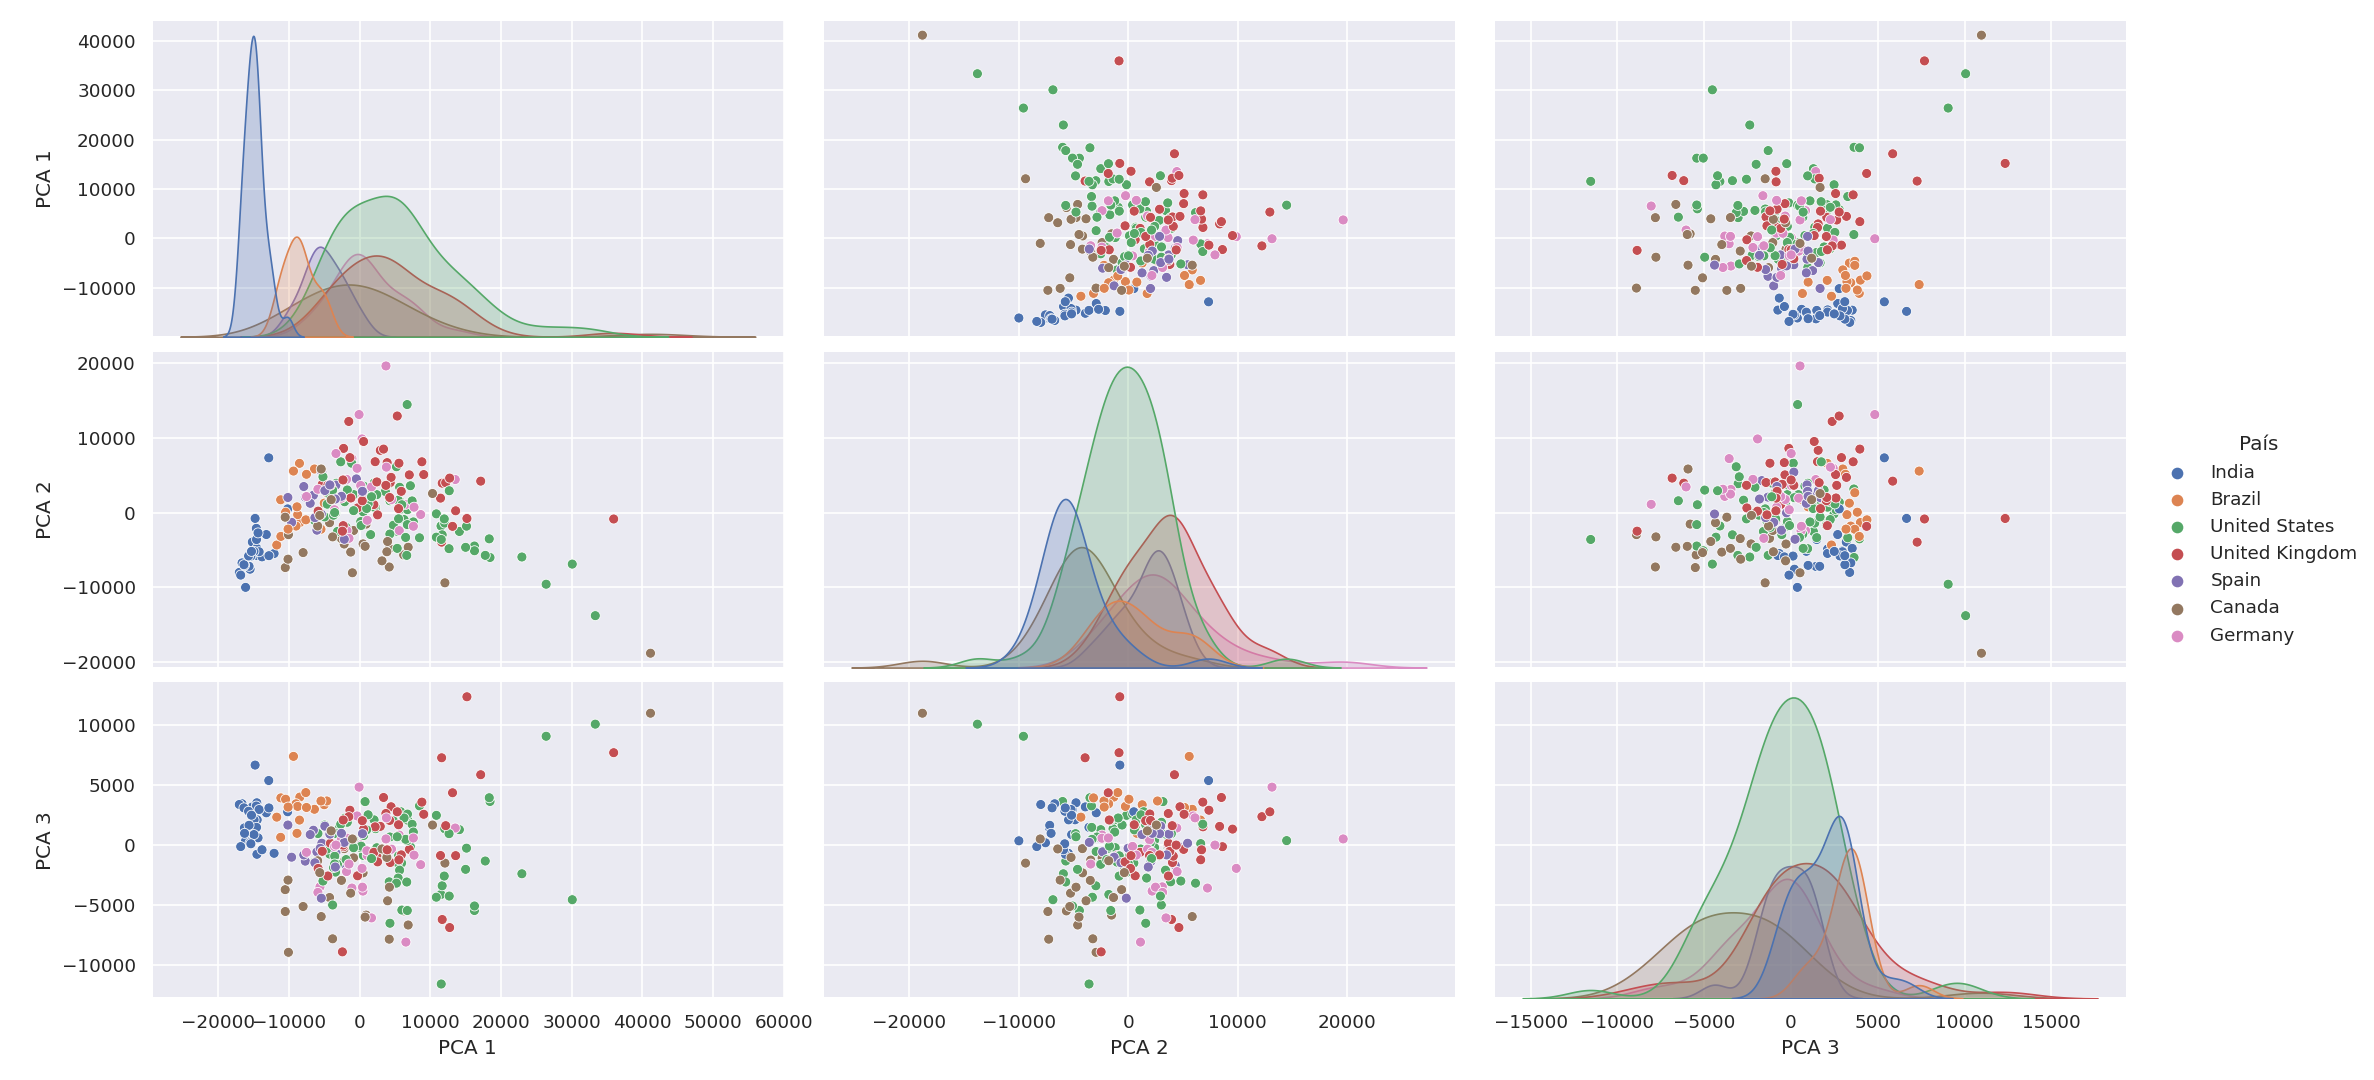
\includegraphics[width=17.2cm]{fig/plotplus.png}
\end{center}
\end{2}

\begin{2} \normalfont Visualização das direções dos autovetores no 3º Plano.

\begin{center}
    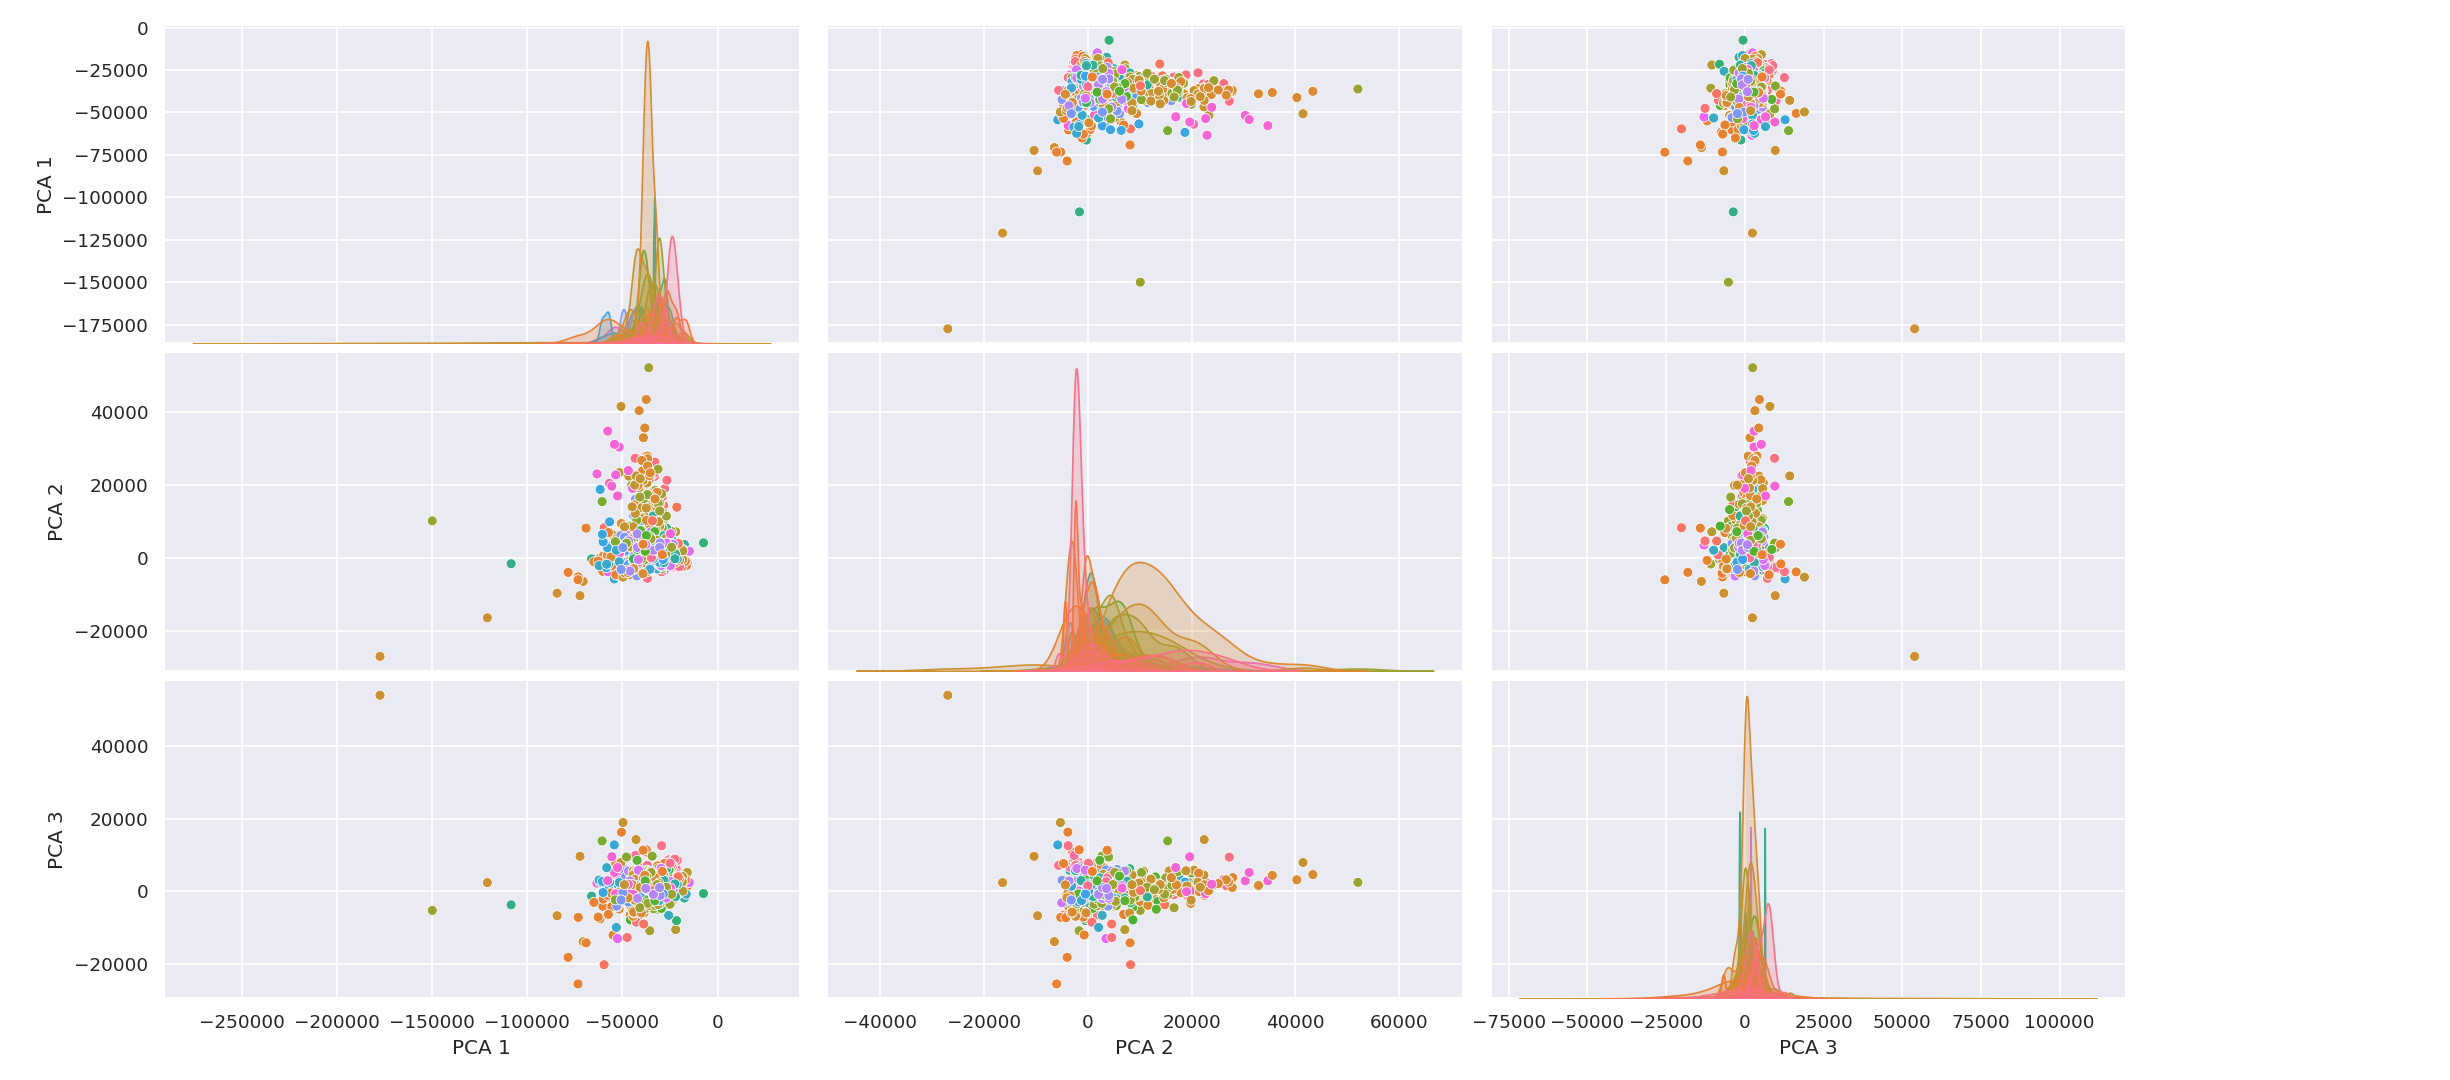
\includegraphics[width=10.8cm]{fig/plot02.png}
\end{center}
\end{2}

\section{Conclusão}

\hspace{0.6cm}Pela utilização dos componentes principais em qualquer análise, logo, temos uma visão multivariada do conjunto de dados, onde cada componente principal, é uma combinação linear das variáveis originais, e pelo primeiro componente principal, tenta explicar a variabilidade máxima do conjunto de dados, e o segundo tenta explicar o restante dela, e assim até o último. Podemos escolher a quantidade de componentes que, pela sua soma, chega perto de 100\%, e pela utilização dos componentes, podemos extrair fatores importantes dos dados e produzir visualizações de dados de diversos planos, entretanto só podemos visualizar até o terceiro plano. Por essa razão a maioria das análises utiliza-se de até 3 componentes.

\end{document}
